\documentclass[a4paper,man,natbib,floatsintext,donotrepeattitle]{apa6}

\usepackage[english]{babel}
\usepackage[utf8x]{inputenc}
\usepackage{amsmath}
\usepackage{graphicx}
\usepackage[colorinlistoftodos]{todonotes}
\usepackage{xcolor}
\usepackage[draft,inline,nomargin,index]{fixme}
\usepackage{hyperref}
\usepackage{verbatim}
\usepackage{nameref}
\usepackage{booktabs}
\usepackage{lineno}
\usepackage{amsfonts}
\usepackage{booktabs}
\usepackage{siunitx}
\linenumbers

\fxsetup{theme=color,mode=multiuser}
\FXRegisterAuthor{ab}{sab}{\color{blue}Amelie} % abnote{} with text inside to edit
\FXRegisterAuthor{bb}{sbb}{\color{purple}Brice} % bbnote{} with text inside to edit
\FXRegisterAuthor{ln}{sln}{\color{violet}Lad} % lnnote{} with text inside to edit

%\title{Blinding as a Necessary Precaution Against Experimenter Biases During Sequential Bayes Factor: A commentary on \cite{schonbrodt_sequential_2017}}

%\title{On the importance of blinding during sequential testing procedures: A commentary on \cite{schonbrodt_sequential_2017}}

%\title{"Efficient" yes, but only if you blind yourself: A commentary on \cite{schonbrodt_sequential_2017}}

%\title{"Efficient", but blind yourself as a precaution: A commentary on \cite{schonbrodt_sequential_2017}}

%\title{Blinding as a Precaution Against Experimenter Biases During Sequential Testing: A commentary on \cite{schonbrodt_sequential_2017}}

\title{Triple Blinding for Sequential Testing: A commentary on \cite{schonbrodt_sequential_2017}}

\shorttitle{Blind Bayes Factor}
\threeauthors{Amélie G. Bret}{Brice Beffara}{Ladislas Nalborczyk}
\threeaffiliations{Univ. Grenoble Alpes, CNRS, LPNC, 38000, Grenoble, France \\ Psychological Science Research Institute, Catholic University of Louvain, Belgium \\ The Walden III Slowpen Science Laboratory, France}{The Walden III Slowpen Science Laboratory, France}{Univ. Grenoble Alpes, CNRS, LPNC, 38000, Grenoble, France \\ Department of Experimental Clinical and Health Psychology, Ghent University \\ The Walden III Slowpen Science Laboratory, France}

\abstract{We discuss potential issues associated with the Sequential Bayes Factor procedure as introduced by \cite{schonbrodt_sequential_2017}. We argue that particular precautions should be undertaken to ensure objectivity during sequential testing procedures (both Bayesian and frequentist). More precisely, we highlight the need for triple-blinding during such procedures, and provide recommendations on how to implement this without additional costs, while taking into account the specificity of the sequential testing situation.}

\keywords{Sequential Bayes Factor, sequential testing, triple-blind, research methods}

% re-enabling section numbering (disabled by the apa6.csl)
% \setcounter{secnumdepth}{3}

\begin{document}

% defining a new command for counting words
\newcommand{\quickwordcount}{%
  \immediate\write18{texcount -1 -sum -merge \jobname.tex > \jobname-words.sum }%
  \input{\jobname-words.sum}words%
}

\maketitle

Wordcount: This document contains \textbf{\quickwordcount}.

\newpage

%\tableofcontents % provisoire, juste pour se repérer entre nous
%\newpage

%%%%%%%%%%%%%%%%%%%%%%%%%%%%%%%%%%%%%%%%
% début du comment
%%%%%%%%%%%%%%%%%%%%%%%%%%%%%

\newpage

\section{Introduction}

\cite{edwards_ward_bayesian_1963} state, "the rules governing when data collection stops are irrelevant to data interpretation. It is entirely appropriate to collect data until a point has been proven or disproven, or until the data collector runs out of time, money, or patience". However, this practice has severe pitfalls in the classical NHST paradigm, as it dramatically increases Type I error rates. \cite{schonbrodt_sequential_2017} say: "Of course, one can calculate statistics during data collection, but the results of these tests must not have any influence on optionally stopping data collection."

We argue that such interim analysis (including visual inspections of the data) might have an influence on future data collection through overlooked experimenter effects, thus biasing the expected results of sequential testing procedures (both Bayesian and frequentist). While the procedure described in \cite{schonbrodt_sequential_2017} offers an attractive perspective on data collection and while we generally agree with most of their recommendations, we draw attention about precautions that need to be undertaken in order to preserve the long-terms rates of wrong inferences they provide. One major concern is that the person who runs the experiment and the person who analyses the data are usually the same person. As noted by \cite{wicherts_degrees_2016}, in the psychological field, "the analyses are typically conducted by a person who is not only aware of the hypotheses, but also benefits directly from corroborating them". Thus, failures of blinding procedures are listed among the 34 researchers degrees of freedom identified by \cite{wicherts_degrees_2016}. In the current commentary we highlight the particular dramatic consequences of blinding failures in the context of sequential testing, and suggest a new way to combine triple blinding with sequential testing, taking into account the specificities of such procedures.

%In their paper, \cite{schonbrodt_sequential_2017} present an alternative to the much used NHST with a priori power analysis (NHST-PA). They introduce the \textit{Sequential Bayes Factor} (SBF) procedure that allows to collect data iteratively, until a predefined threshold is reached, while not suffering from the pitfalls associated with similar procedures used in the NHST framework. Testing mean differences between two independent groups, they show that the SBF design typically needs 50\% to 70\% smaller samples to reach a conclusion about the presence of an effect, as compared with optimal NHST-PA (where \textit{optimal} stands for an idealized situation in which the a priori targeted effect would be exactly equal to the \textit{true} effect size), while having similar long-term error rates.

\section{Intrapersonal and interpersonal biases in SBF procedure}

When a data analyst has expectations about what should be observed, data analysis is likely to be biased by these expectations trough confirmation (favoring an hypothesis) or disconfirmation (stronger skepticism toward data against the hypothesis than toward data corroborating the hypothesis) biases \citep{lilienfeld_blind_2017}. When an experimenter has expectations about what should be observed, data collection is likely to be biased by these expectations \citep{orne_social_1962,rosenthal_social_1963,rosenthal_experimenter_1964,tuyttens_opinion_2016,zoble_interaction_1969}.
In this comment, we discuss sequential testing assuming that both the participant and the experimenter are blind to the experimental condition (double blind design). In less rigorous conditions (simple blind or even no blinding at all), more problems can arise from sequential testing. \par

What is the specific status of sequential testing concerning analyst and observer expectancy effects ? Expectancy effects arise when one has prior beliefs and/or motivations about the issue of an experiment and involuntarily (we assume scientific honesty) influences the results on the basis of these prior beliefs and motivations. The confidence toward an hypothesis can be influenced by previous results from the literature, naive representations about the studied phenomenon, and all other sources of information. All these sources of information may deal with the studied phenomenon but rarely with the ongoing study specifically. As a consequence, the confidence about an hypothesis is always subject to uncertainty. When performing sequential testing, one has a direct access to accumulation of evidence concerning the ongoing study. As a consequence, the prior information is far more certain than previous studies or naive representations. Hence, the risk to fall into an "evidence confirmation loop" is increased. This risk applies both to confirmation and disconfirmation biases (data analysis), and observer expectancy effects (data collection). During data analysis, the intrapersonal bias of data evaluation can inflate with accumulated evidence. During data collection, the interpersonal bias of experimenter-participant interaction can inflate with accumulated evidence. However, the interpersonal bias is probably more important (more channels of influence), and we will therefore focus on it. \par

%\begin{figure}[H]
%  \caption{Overview of the SBF procedure and illustration of potential biases when the experimenter and the data analyst are the same person.}
%  \centering
%  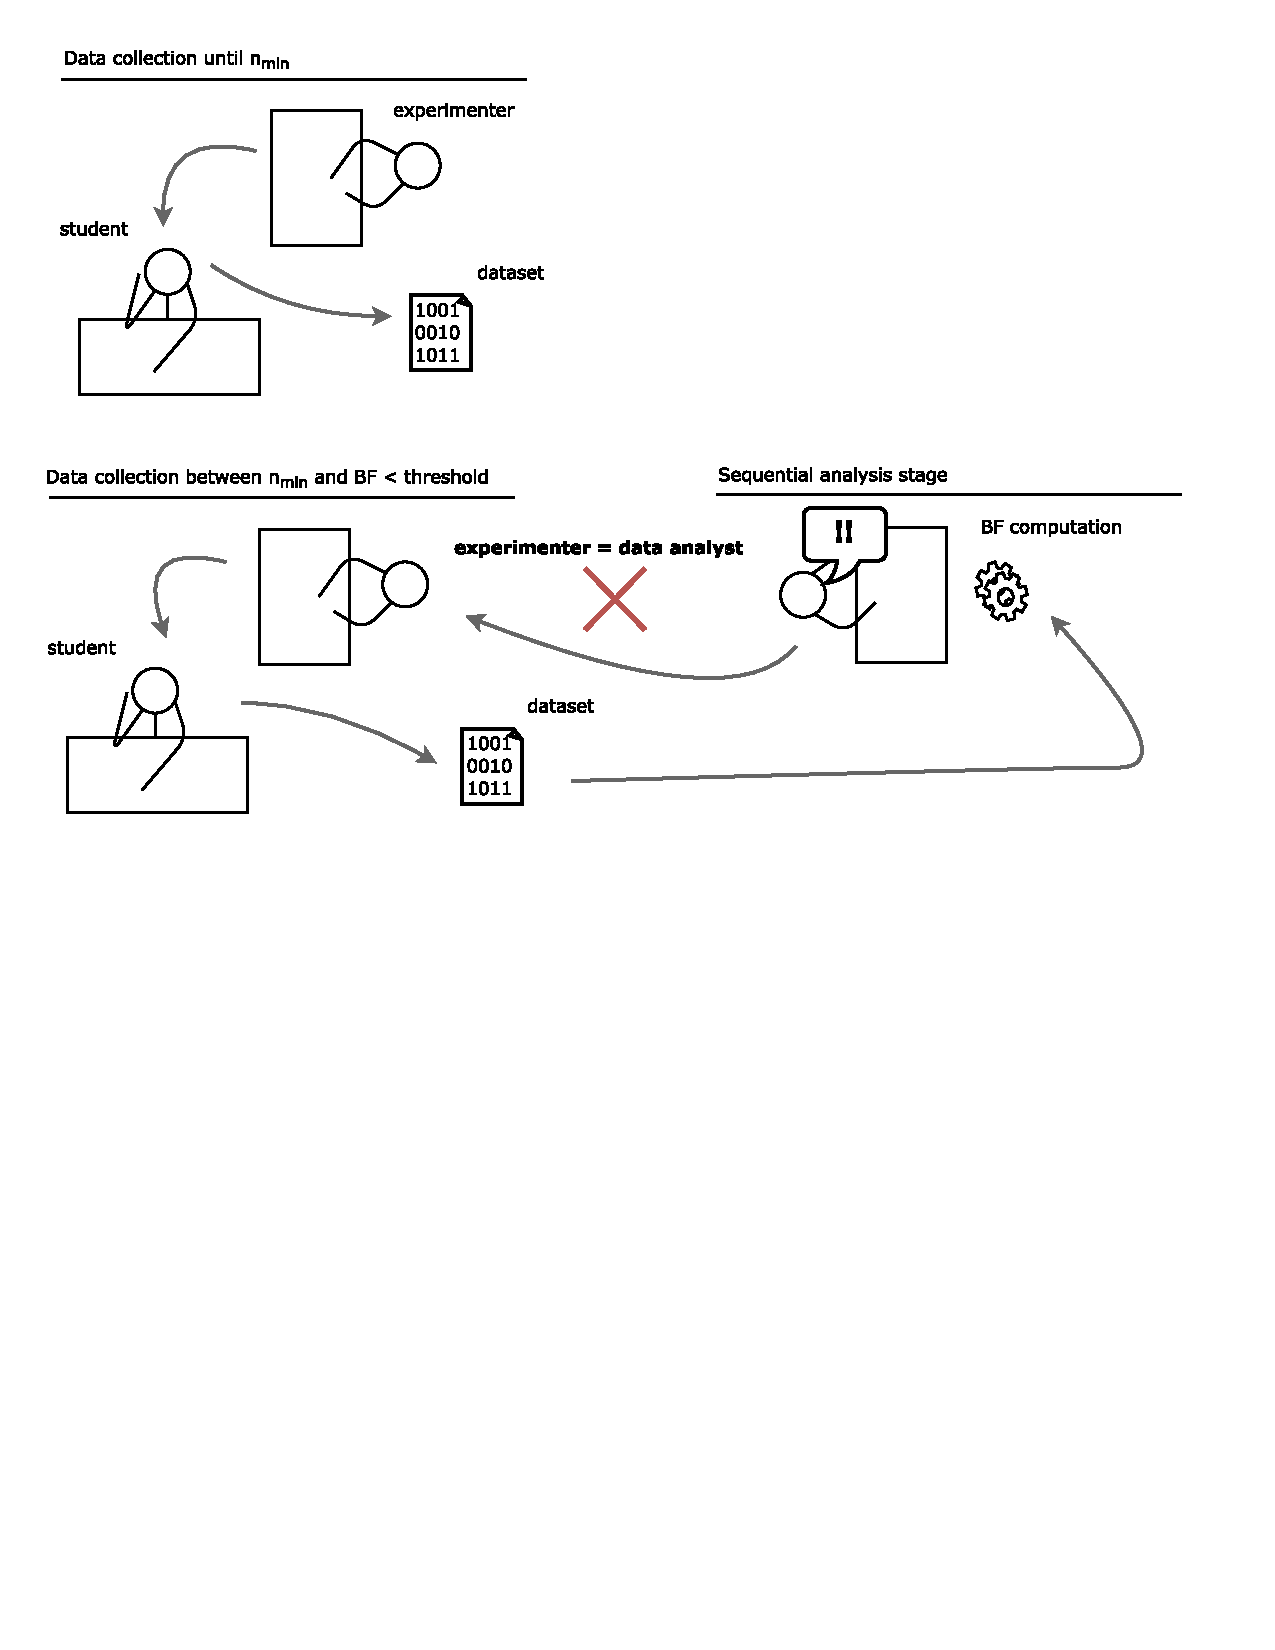
\includegraphics[width=0.8\textwidth]{figures/bias_diag.pdf}
%  \label{fig:diag1}
%\end{figure}

Obviously, It is very hard to obtain robust results concerning the effect size of analyst and observer expectancy effects. This ("meta-science") problem \lnnote{je pense qu'on peut le dire autremenent, mais je n'ai pas mieux pour le moment...peut-être simplement "methodological problem" ? ou alors simplement enlever "meta-science" de la phrase ?} is complicated because these biases can apply at all the levels as one experiment is included in another. It is also difficult to collect large observation samples by experimental conditions \citep[e.g.,][]{zoble_interaction_1969}. Thus, we can only draw attention to these effects as a potential risk to consider rather than as a robust and clearly identified danger to avoid. \par

Because we assume a double blind design, how could knowledge about the data influence the issue of the experiment ? It is possible that the experimenter's verbal and non-verbal motor cues impact the participant's behavior \citep{zoble_interaction_1969}. In a double-blind design, the experimenter cannot influence the participant's responses on the basis of the experimental condition knowledge. However, the (de)motivation and the disappointment/satisfaction of seeing the preferred hypothesis contradicted/confirmed by the sequential testing procedure can influence the participant. We cannot exclude that the confidence in an hypothesis can interact with experimental conditions and impacts the issue of the experiment in one way or another.\par

Let's take a quick fictitious example. We want to study the effects of working memory (WM) training on math performance. We compare a WM training effect with a control group (e.g., short memory training) on a math test. Either in a between or a within participant design, let's imagine that there is a true effect of WM training on math performance (H1). With accumulation of evidence in this direction, if the experimenter is not blind to sequential testing procedure (and let's say pro H1), it is likely that he or she will show higher enthusiasm when interacting with (e.g., delivering instruction to) the participant. The participant will in turn likely wish to perform the experiment at best \citep{zoble_interaction_1969}. The WM training is expected to increase performance at the math test. It is then possible to observe an interaction between the motivation of the experimenter and the treatment effect, with increased motivation perceived during instructions explanations amplifying the positive effect of treatment. Importantly, this kind of bias can emerge in all combinations of a priori expectations and hypothesis truth (see Table \ref{tab:pred}). \par

%\vline

%\begin{table}
%  \centering
%	\begin{tabular}{SSSS} \toprule
%     & \textbf{True} & & \\ 
%    \textit{Expected} & {effect} & \textit{H0} & \textit{H1} \\ \midrule
%     & \textbf{H0} & {+H0} & {-H0} \\
%     & \textbf{H1} & {-H1} & {+H1} \\ \bottomrule 
%	\end{tabular}
%    \caption{Possible interactions between true and expected effect on its %observation. + = accelerate and - = decelerate convergence.} %\label{tab:hexp}
%\end{table}
%\par

\vspace{5mm}

\begin{table}[H]
\centering
\caption{Possible interactions between population effect size and a priori beliefs during a sequential testing procedure. Congruent observations are expected to increase the speed of threshold reaching (H0+ and H1+), while incongruent observations are expected to slow down the process (H0- and H1-), and to increase the number of false alarms.}
\label{tab:pred}
\resizebox{\textwidth}{!}{%
\begin{tabular}{@{}ccc@{}}
\toprule
 & \begin{tabular}[c]{@{}c@{}}There is no difference in the population\\ (H0, $\delta = 0$)\end{tabular} & \begin{tabular}[c]{@{}c@{}}There is a difference in the population\\ (H1, e.g., $\delta = 0.5$)\end{tabular} \\ \midrule
Researcher 1, believes in H0 & H0+ (congruent) & H0- (incongruent) \\
Researcher 2, believes in H1 & H1- (incongruent) & H1+ (congruent) \\ \bottomrule
\end{tabular}%
}
\end{table}

Again, evidence is insufficient to conclude that analyst and observer expectancy effects are absolutely necessary to take into account. If the cost of reducing the bias was high, we could be skeptical about considering it, knowing its uncertain benefits. However, as we will suggest in the next section, very easy to implement and costless methods can be applied to overcome these biases. Hence, even with low certainty about the risks, it is worthwhile to limit it all the same. \par

% Sequential-Experimenter-Analyst-Bias (SEAB)...direct consequence of the SEAB is that it introduces a time dependency between participants...this kind of auto-correlated data would invalidate the use of the models compared by...in their original paper...

These biases can wear a multitude of forms as it is a function of the researcher \textit{a-priori} expectancies and of the population effect size. Moreover, we focus here on the simplest case in which the expectancies of the researcher remain constant throughout the sequential testing procedure. Although probably non realistic, this setting serves illustrative purposes. Figure \ref{fig:pred} illustrates our predictions concerning the biased evolution of Bayes Factor during sequential testing, according to the four situations presented in Table \ref{tab:pred}. The main message is that congruent situations (i.e., H0+ and H1+) would make the predefined boundary faster to reach (i.e., the sample size at which the boundary is hit would be lower than usually) and would lower error rates, while incongruent situations (i.e., H0- and H1-) would slow down this process and increase error rates.

\begin{figure}[H]
  \caption{Predicted consequences on the result of a SBF procedure with a fixed boundary of BF10 = 6 (or BF10 = 1/6), for a given Cohen's d of 0.5 (hereafter, "H1") or of 0 (hereafter "H0"), and according to the \emph{a priori} researcher expectancies.}
  \centering
  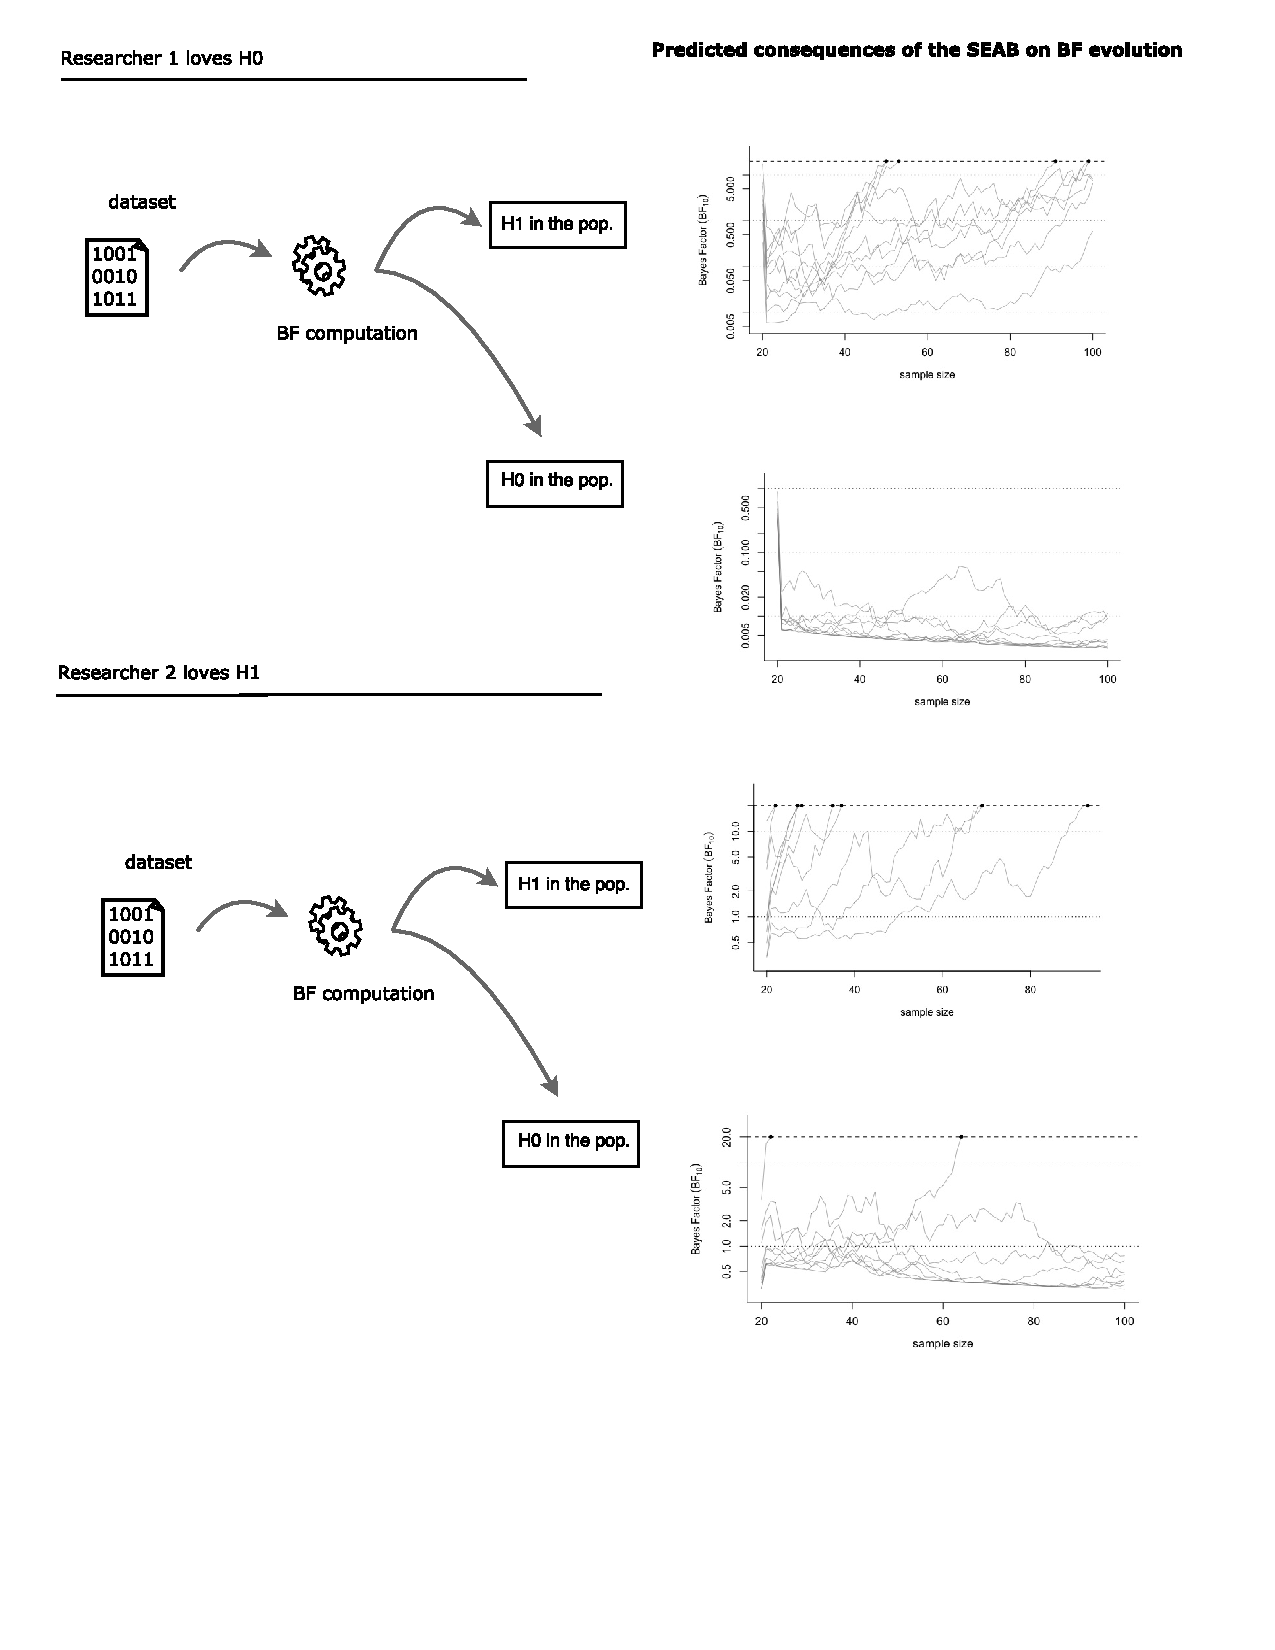
\includegraphics[width=0.8\textwidth]{figures/BFF_predictions.pdf}
  \label{fig:pred}
\end{figure}

Having presented the mechanisms through which we expect the knowledge of previous data to influence the data collection process, and illustrated the predicted consequences of these biases on the evolution of sequentially computed Bayes Factors, we focus on the next section on how to prevent this to happen. We suggest two ways of implementing triple blinding as a precaution against experimenter biases during sequential testing, and present the concepts of an automated procedure that would ensure objectivity.

\section{Solutions ? Blind yourself.}

\subsection{Solution 1: one analyst, one experimenter}

%Hence, we suggest doing triple blinding is which participants, experimenter and data analyst are not aware of the experimental informations (conditions, hypothesis...)

Double blinding advantages is now well documented \citep{schulz_blinding_2002}, however, this procedure does not allow to answer the problem of experimenter effect in the SBF procedure. Although double blinding procedures have became a gold standard in many psychological fields, much less attention has been dedicated to triple blinding (i.e., procedures ensuring that the person who analyses the data is blinded to hypotheses). Triple blinding has first been applied with great success in clinical trials, where \textit{triple} refers to the fact that the committee who assess the results of a trial is blind to the hypothesis. Applied to data analysis, triple blinding refers to a situation in which data analysis is performed by an individual who is not aware of the hypotheses and thus, who has not particular interest in corroborating or disproving it \citep{miller_blind_2011}. This practice, while not largely spread in psychology, would be a remedy for many of the biases identified in \cite{wicherts_degrees_2016}. However, we understand that it is a luxury possibility and it is not easy to apply, mostly due to materials and time constrains.

\subsection{Solution 2: one analyst-experimenter, "software-blinded"}

Another solution is to automate triple blinding, so that the data analyst (which can be the experimenter) is blinded to the Bayes Factors computed on previous observations. As an example on how to implement this idea, we added a very short append to the \texttt{seqBF} function, written by Félix Schönbrodt \& Richard Morey (available \href{https://raw.githubusercontent.com/richarddmorey/BayesFactorExtras/master/BayesFactorExtras/R/seqBF.R}{here}), so that the user can now simply set the \texttt{blind} argument to \texttt{TRUE} and thus be completely blind to the results of the SBF procedure. The only output is a sentence that either indicates to "continue" or to "stop" the recruitment, considering an a-priori defined threshold (see \nameref{sec:supp} for code details). The main advantage of this solution is that it's a costless and ready-to-use solution. However, we suggest in the following section a more complete treatment of the biases that can emerge during sequential testing by sketching the main ideas of an automated triple blinding procedure that takes into account the specificities of sequential testing procedures.

\subsection{Full automation of data analysis}

When sequentially computing a BF, we are faced with many choices about how to deal with new incoming data. Based on previous studies, we might have expectations about the range of plausible values, the need for re-coding or transforming data, or the distribution of residuals. All these decisions should be made before starting the SBF procedure, in order not to be contaminated by the previously discussed biases. In a triple blind perspective, we propose that all these treatments should be automated and performed at each step of the sequential testing procedure. This way, outliers data processing (for instance) would be done in an incremental manner, with the entire dataset always reconsidered - including former outliers -, so that this process would follow the progressive incorporation of new observations (i.e., such a procedure should be able to take into account that an extreme observation at time \textit{t} might not be extreme anymore at time \textit{t+n}). The fact that this iterative procedure is automated should prevent the data analyst from classical traps during data manipulation. Theses traps could have much more dramatic consequences in SBF in comparison to traditional procedures due to the incremental nature of the expectancy effects. Besides, this idea fits well with the open science philosophy and with preregistration practices. Indeed, we propose that these steps would be programmed and coded on the basis of preregistered choices, before starting to collect data. Triple blind designs with automated data analysis would therefore ensure the error rates of empirical SBF procedures to be similar to the long-term error rates provided by \cite{schonbrodt_sequential_2017} using simulation, and explicitly fulfill the requirements of transparent and reproducible science. \par

%\subsection{Experimental demonstration}
%After Rosenthal's studies, the effect of experimenter influence in the experiment have not been studied a lot. Because of this lack of knowledge, and of the hypothetical importance in the SBF, we suggest a simple design to test the experimenter bias. Following the Figure 2. In one condition, we would say the experimenter that the effect is congruent with H0... One group without any SEAB correction, and the second one with a triple blind or a software-blind.

\section{Conclusions}

%We acknowledge that only a few and non recent papers have highlighted experimenters biases, but we think that we can not take the risk with a so highly rigorous procedure to add any social bias \lnnote{je ne suis pas certain de comprendre la deuxième partie de cette phrase... c'est le SBF qui est rigorous ? why ?}. Combining both of those procedures (SBF and triple blinding) could, in our view, increase again the transparency and the rigor of research. With this comment we would like to point out the importance of SBF procedure when it is combined with a blinding procedure, but maybe even more the importance of a global approach of automaticity and blinding \lnnote{what do you mean ?}. In this vein, our proposal is somehow similar to the \textit{born-open data} proposal of \cite{rouder_what_2016}...

We proposed a straightforward approach for triple blind designs while using sequential testing. Although the magnitude of intrapersonal and interpersonal biases is uncertain in data analysis and data collection, triple blinding is a costless security likely to increase the transparency and reliability of data analysis. Due to its specific status, sequential testing could benefit from triple blinding even more than traditional analysis methods. Triple blinded sequential testing could improve hypothesis testing within the "costs and benefits trade-off" world of the researcher.

\section{Supplementary materials}\label{sec:supp}

Reproducible code and supplementary materials can be found on OSF: \url{osf.io/mwtvk
}.

\section{Acknowledgements}

...

\bibliography{BBF}

\end{document}
